\documentclass{beamer}
\usepackage{amsmath}
\usepackage{rotating}
\usepackage{graphicx}
\usepackage{multimedia}

\useinnertheme[shadow=true]{rounded}
\useoutertheme{shadow}
\usecolortheme{orchid}
\usecolortheme{whale}

\mode<presentation>

\newcommand{\dif}{\, \mathrm{d}}
\newcommand{\diff}[2]{\frac{\mathrm{d}#1}{\mathrm{d}#2}}
\newcommand{\partdiff}[2]{\frac{\partial #1}{\partial #2}}


\title{TMA4280 - Introduction to supercomputing}
\subtitle{Past, current and future supercomputers}
\author{Einar M. R{\o}nquist and Arne Morten Kvarving}
\institute{NTNU and SINTEF ICT}
\date{January 2011, revised December 2011}

\begin{document}

\maketitle


\begin{frame}\frametitle{Top 500 systems}
\begin{center}
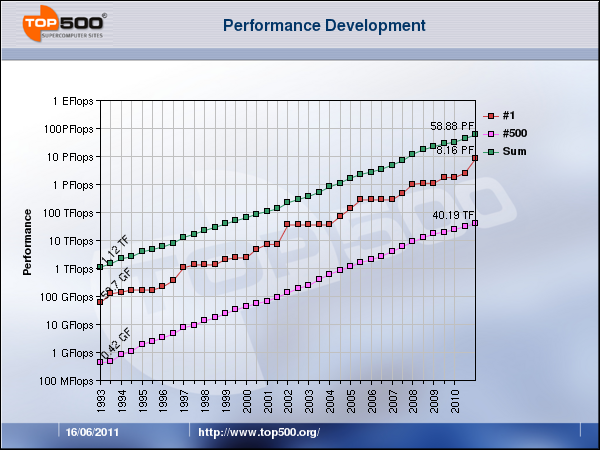
\includegraphics[width=10cm]{Performance_Development}
\end{center}
\end{frame}

\begin{frame}\frametitle{Top 500 systems}
\begin{center}
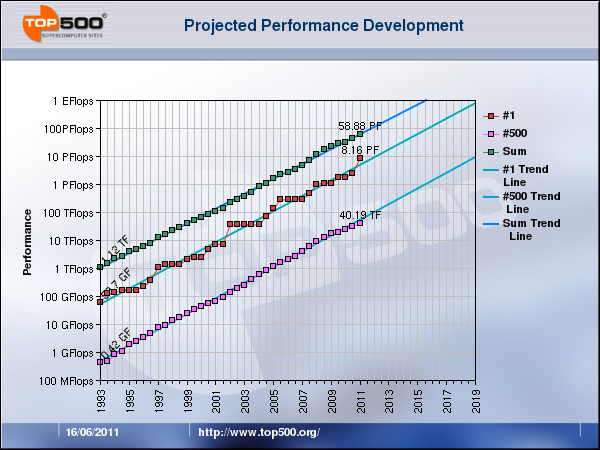
\includegraphics[width=10cm]{Projected_Performance_Development}
\end{center}
\end{frame}

\begin{frame}\frametitle{Supercomputers at NTNU}
A supercomputing center was established in 1986
\vspace{.2in}

\begin{tabular}{|l|l|l|l|l|l|}
\hline
Year & System & \#proc & type & GF (*)\\
\hline
1986-1992 & Cray X-MP & 2 & vector & 0.5 \\
1992-1996 & Cray Y-MP & 4 & vector & 1.3\\
1995-2003 & Cray J90     & 8 & vector & 1.6 \\
1992-1999 & Intel Paragon & 56 & MPP & 5.0\\
1996-2003 & Cray T3E & 96 & MPP & 58\\
2000-2001 & SGI O2 & 160 & CCNUMA & 100\\
2001-2008 & SGI O3 & 898 & CCNUMA & 1000\\
2006-2011 & IBM P5+ & 2976 & distributed SMP & 23500\\
2012-     & SGI Altix ICE X & 23040 & distributed SMP & 497230 \\
\hline
\end{tabular}

\vspace{.5in}
%(*)   several upgrades; currently 512 processors left\\
(*) maximum theoretical performance in Gflops
\end{frame}



\begin{frame}\frametitle{Previous supercomputer at NTNU}
\begin{center}
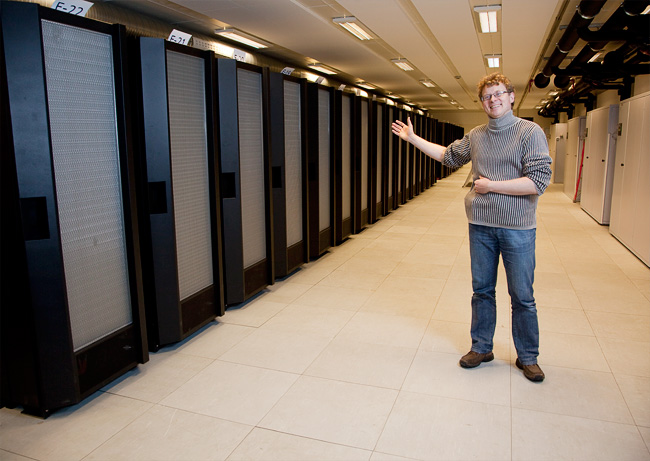
\includegraphics[width=9cm]{njord_john}
\end{center}
njord @ NTNU: 3000 processors
\end{frame}

\begin{frame}\frametitle{Current supercomputer at NTNU: {\em vilje}}
\begin{itemize}
\item Full name: \texttt{vilje.hpc.ntnu.no}
\item System: SGI Altix ICE
\item Type: distributed SMP 
\item Number of nodes: 1440
\item A single node: \\
a shared memory system; 2 octa-core chips; 32 GB memory
\item Number of cores (physical): 23040
\item Number of cores (logical): 46080
\item CPU type: Intel Sandy Bridge
\item Theoretical total peak: 479.23 Tflops
\item Weight: This machine is shy and refuse to tell me.
\end{itemize}
\end{frame}


\begin{frame}\frametitle{Previous supercomputer at NTNU: {\em njord}}
\begin{center}
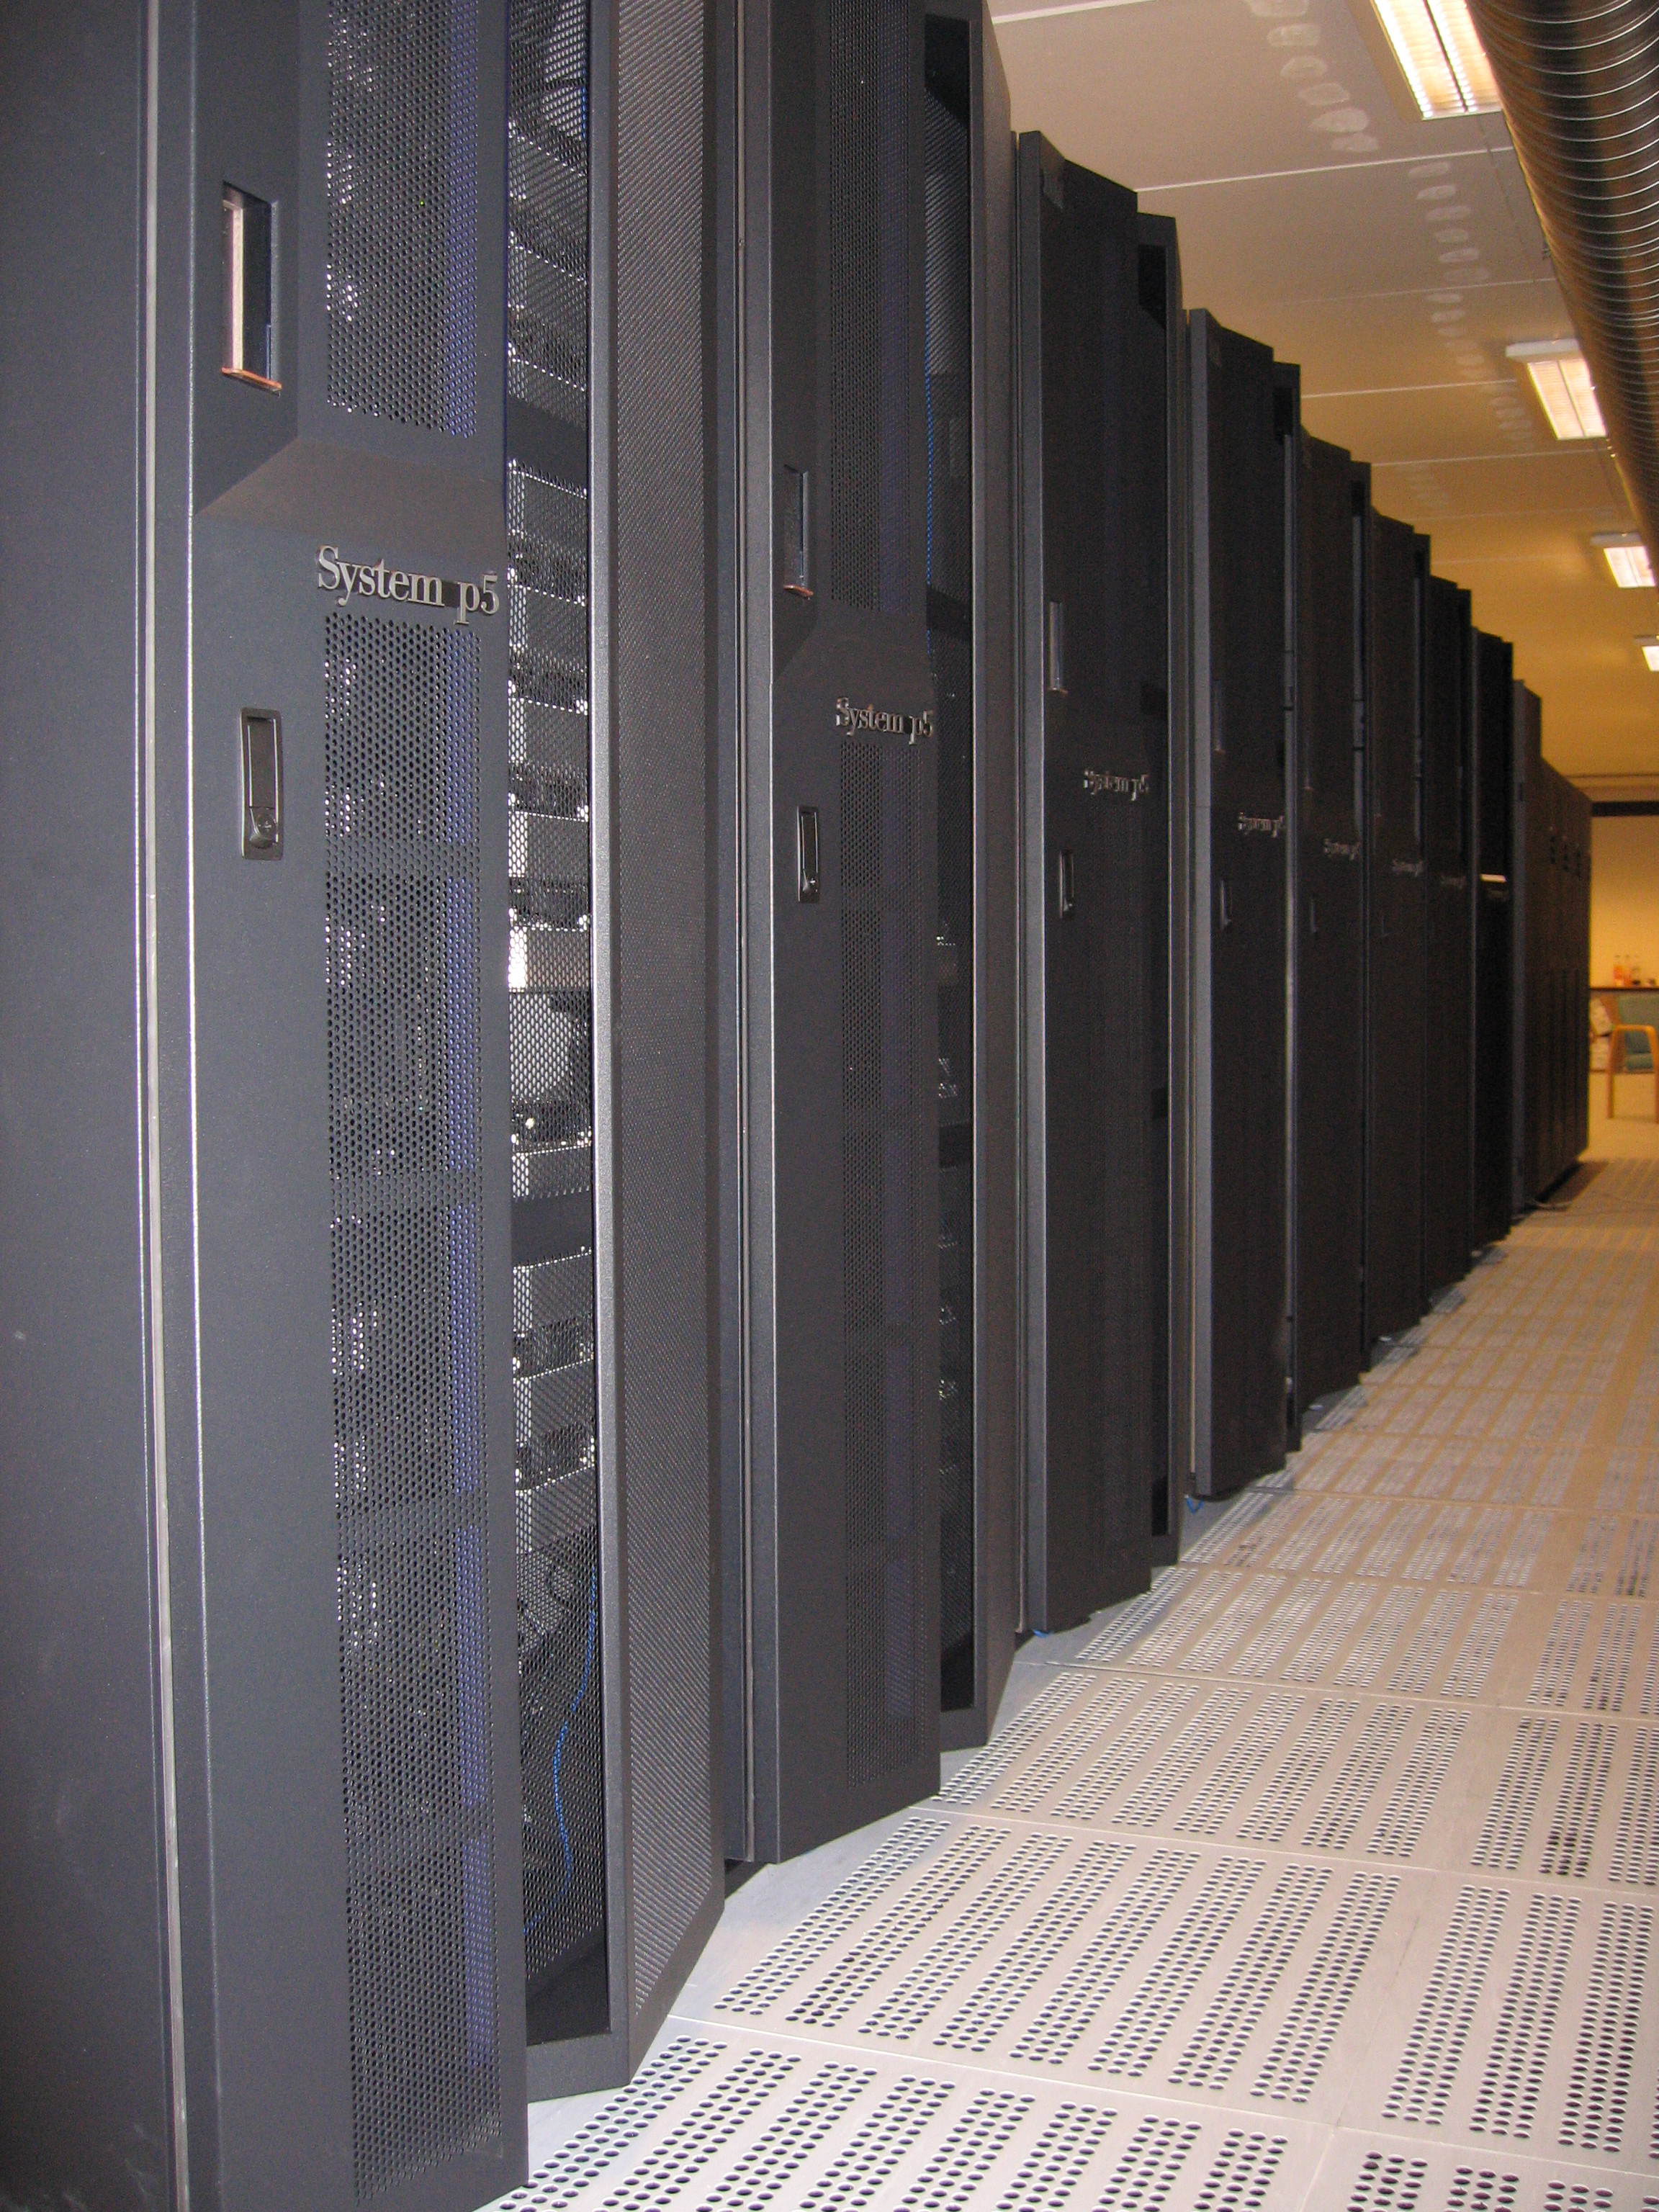
\includegraphics[width=6cm]{njord_1}
\end{center}
\end{frame}

\begin{frame}\frametitle{Example of use: weather forecasting}
\begin{center}
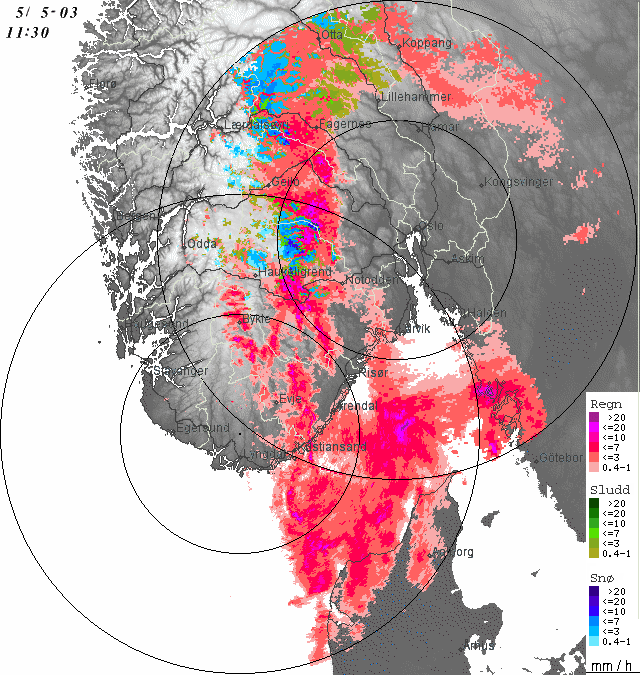
\includegraphics[width=6cm]{met}
\end{center}
For more information, see \texttt{http://met.no}
\end{frame}

\begin{frame}\frametitle{Example of use: turbulence prediction}
\begin{center}
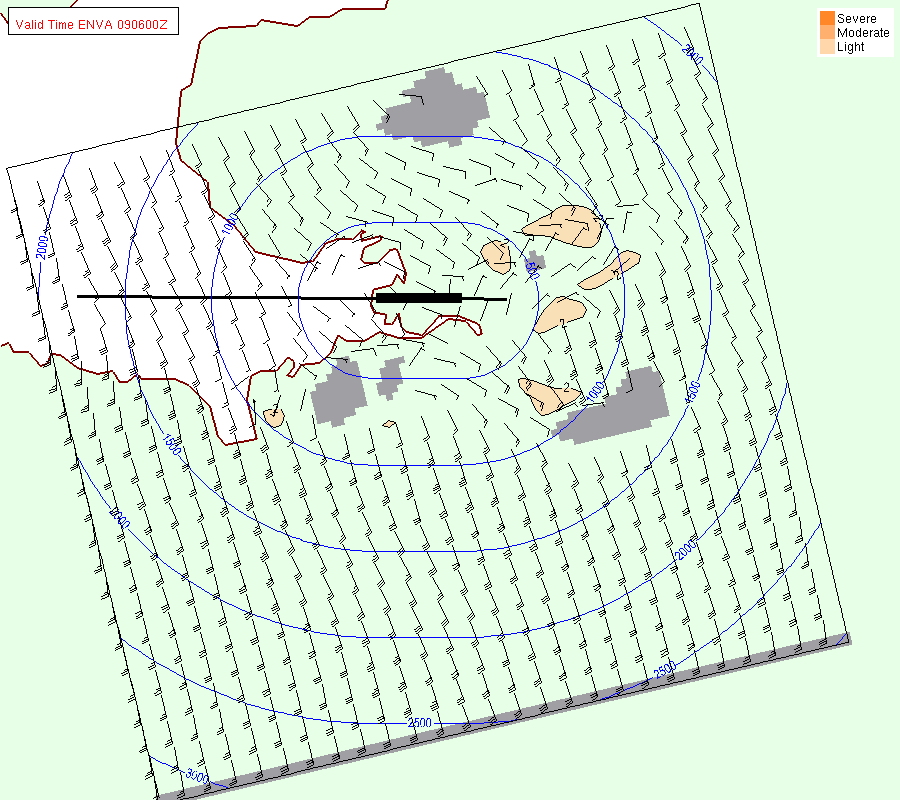
\includegraphics[width=6cm]{simra}
\end{center}
For more information, see \texttt{http://ippc.no} \\
\texttt{http://sintef.no/Projectweb/WindModeling/Projects/Avinor/}
\end{frame}

\begin{frame}\frametitle{Example of use: climate modelling}
\begin{center}
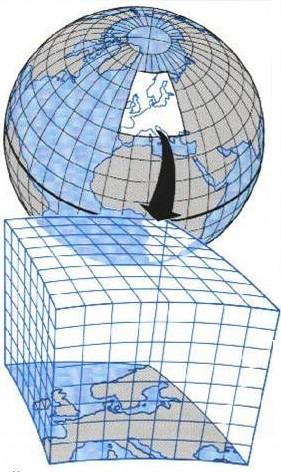
\includegraphics[width=3cm]{climate_model}
\end{center}
For more information, see \\
\texttt{http://www.bcm.uib.no} and \\
\texttt{http://www.bjerknes.uib.no}
\end{frame}

\end{document}


